\documentclass[]{article}
\usepackage{graphicx}
\usepackage{hyperref}

%opening
\title{Assignment 2 CDA}
\author{Tim van Rossum, 4246306\\
	Michiel Doesburg, 4343875}

\begin{document}

\maketitle
\section{Familiarization with the data}
The dataset contains a total of 44 signals, with some being static values, other being sinusoid signals, and others being partially discrete (as in, they can rise or drop at certain points). L-signals tend to be more sinusoidal, F-signals tend to be "partially discrete", and S-signals are all binary signals.

All the signals together seem to have little correlation. Some combinations of signals are reasonably correlated: e.g. L\_T3 and P\_J302 have a 0.42 correlation coefficient. 

\begin{figure}

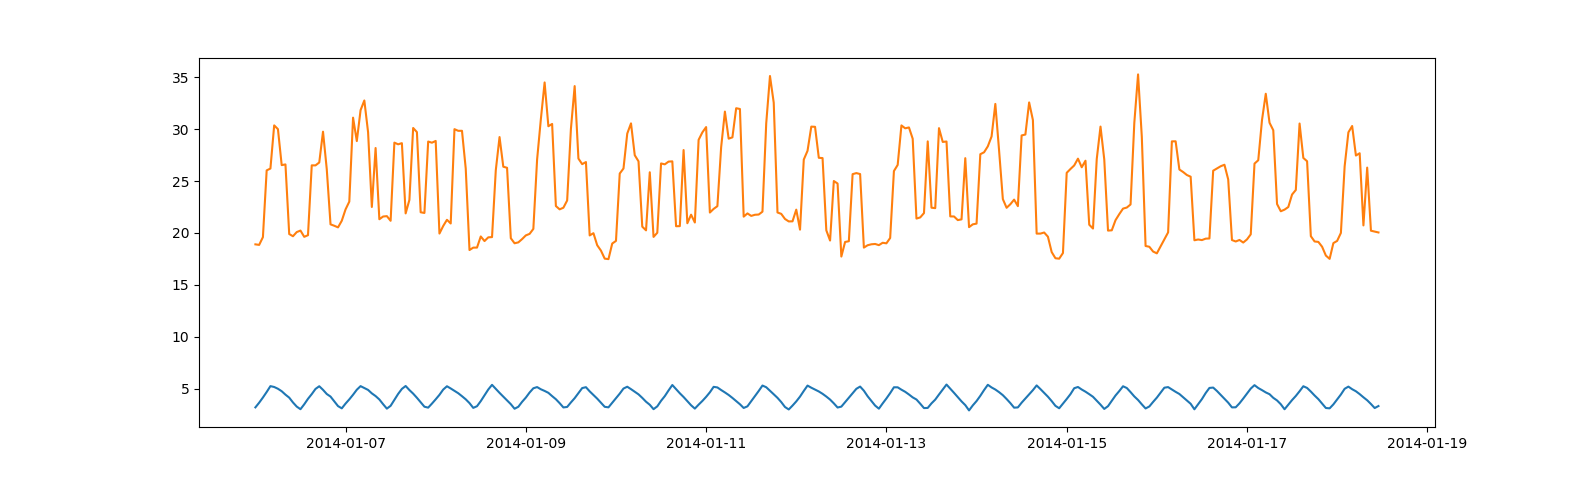
\includegraphics[width=10cm,height=8cm]{./visuallizations/correlated_signals.png}.
\caption{Signals L\_T3 and P\_J302. The peaks are roughly aligned.}
\end{figure}
\end{document}
